%%%%%%%%%%%%%%%%%%%%%%%%%%%%%%%%%%%%%%%%%
% Beamer Presentation
% LaTeX Template
% Version 1.0 (10/11/12)
%
% This template has been downloaded from:
% http://www.LaTeXTemplates.com
%
% License:
% CC BY-NC-SA 3.0 (http://creativecommons.org/licenses/by-nc-sa/3.0/)
%
%%%%%%%%%%%%%%%%%%%%%%%%%%%%%%%%%%%%%%%%%

%----------------------------------------------------------------------------------------
%	PACKAGES AND THEMES
%----------------------------------------------------------------------------------------

\documentclass{beamer}

\mode<presentation> {

% The Beamer class comes with a number of default slide themes
% which change the colors and layouts of slides. Below this is a list
% of all the themes, uncomment each in turn to see what they look like.

%\usetheme{default}
%\usetheme{AnnArbor}
%\usetheme{Antibes}
%\usetheme{Bergen}
%\usetheme{Berkeley}
%\usetheme{Berlin}
%\usetheme{Boadilla}
%\usetheme{CambridgeUS}
%\usetheme{Copenhagen}
%\usetheme{Darmstadt}
%\usetheme{Dresden}
%\usetheme{Frankfurt}
%\usetheme{Goettingen}
%\usetheme{Hannover}
%\usetheme{Ilmenau}
%\usetheme{JuanLesPins}
%\usetheme{Luebeck}
\usetheme{Madrid}
%\usetheme{Malmoe}
%\usetheme{Marburg}
%\usetheme{Montpellier}
%\usetheme{PaloAlto}
%\usetheme{Pittsburgh}
%\usetheme{Rochester}
%\usetheme{Singapore}
%\usetheme{Szeged}
%\usetheme{Warsaw}

% As well as themes, the Beamer class has a number of color themes
% for any slide theme. Uncomment each of these in turn to see how it
% changes the colors of your current slide theme.

%\usecolortheme{albatross}
%\usecolortheme{beaver}
%\usecolortheme{beetle}
%\usecolortheme{crane}
%\usecolortheme{dolphin}
%\usecolortheme{dove}
%\usecolortheme{fly}
%\usecolortheme{lily}
%\usecolortheme{orchid}
%\usecolortheme{rose}
%\usecolortheme{seagull}
%\usecolortheme{seahorse}
%\usecolortheme{whale}
%\usecolortheme{wolverine}
\usepackage{mathrsfs}



%\setbeamertemplate{footline} % To remove the footer line in all slides uncomment this line
%\setbeamertemplate{footline}[page number] % To replace the footer line in all slides with a simple slide count uncomment this line

%\setbeamertemplate{navigation symbols}{} % To remove the navigation symbols from the bottom of all slides uncomment this line
}
\usepackage{CJKutf8}
\usepackage{graphicx} % Allows including images
\usepackage{booktabs} % Allows the use of \toprule, \midrule and \bottomrule in tables

% UTF-8 encoding
% CJKfonts package
% latex+dvips, latex+dvipdfm(x) or pdflatex


\AtBeginSection[]
{
	\begin{frame}<beamer>
		\frametitle{Outline for section \thesection}
		{\scriptsize \tableofcontents[ currentsection ]}
	\end{frame}
}
%\tableofcontents[ 
%currentsubsection, 
%hideothersubsections, 
%sectionstyle=show/hide, 
%subsectionstyle=show/shaded, 
%]
\begin{document}
\begin{CJK*}{UTF8}{bsmi}

%\documentclass{article}
%----------------------------------------------------------------------------------------
%	TITLE PAGE
%----------------------------------------------------------------------------------------

\title[KEEL Data-Mining Software Tool]{KEEL Data-Mining Software Tool: Data Set Repository, Integration of Algorithms and Experimental Analysis Framework} % The short title appears at the bottom of every slide, the full title is only on the title page

\author{鍾岳峰} % Your name
\institute[Yue-Fong,Chung] % Your institution as it will appear on the bottom of every slide, may be shorthand to save space
{
元智大學 \\ % Your institution for the title page
\medskip
\textit{pchomekimojuf@gmail.com} % Your email address
}
\date{\today} % Date, can be changed to a custom date



\begin{frame}
\titlepage % Print the title page as the first slide
\end{frame}



\begin{frame}{Outline}
%\begin{frame}[allowframebreaks]{Outline}
\frametitle{Overview} % Table of contents slide, comment this block out to remove it

\tableofcontents[hideallsubsections] % Throughout your presentation, if you choose to use \section{} and \subsection{} commands, these will automatically be printed on this slide as an overview of your presentation
%\framebreak
%\tableofcontents{2}
\end{frame}

%----------------------------------------------------------------------------------------
%	PRESENTATION SLIDES
%----------------------------------------------------------------------------------------

%------------------------------------------------
\section{INTRODUCTION} % Sections can be created in order to organize your presentation into discrete blocks, all sections and subsections are automatically printed in the table of contents as an overview of the talk
%第一章介紹
%------------------------------------------------


%提示%%%%%%%%%%%%%%%%%%%%%%%%%%%%%%%%%%%%%
%****要做重點劃紅線可以用
%{\color{red}fuzzy measures} 
%****草寫
% \Large $\mathscr{B}$
%換行
%\\
%提示%%%%%%%%%%%%%%%%%%%%%%%%%%%%%%%%%%%%%

%------------------------------------------------
%\subsection{INTRODUCTION}
\begin{frame}
	\frametitle{\insertsection : \insertsubsection}
	
	\begin{itemize}
		\item KEEL pays special attention to the implementation of evolutionary learning and soft computing based techniques for \textbf{Data Mining} problems including regression, classification, clustering, pattern mining and so on.
		
		\item The aim of this paper is to present \textbf{three new aspects of KEEL}: \textbf{KEEL-dataset}, a data set repository which includes the data set partitions in the KEEL format and shows some results of algorithms in these data sets;\textbf{ some guidelines for including new algorithms in KEEL}, helping the researchers to make their methods easily accessible to other authors and to compare the results of many approaches already included within the KEEL software; and \textbf{a module of statistical procedures developed} in order to provide to the researcher a suitable tool to contrast the results ob- tained in any experimental study.
		
	\end{itemize}
	
\end{frame}

%------------------------------------------------

%------------------------------------------------

\begin{frame}
	\frametitle{\insertsection : \insertsubsection}
	\begin{itemize}
		\item \textbf{Data Mining (DM)} is the process for automatic discovery of high level knowledge by obtaining information from real world, large and complex data sets [26], and is the core step of a broader process, called \textbf{Knowledge Discovery from Databases (KDD)}.
		\item \textbf{Evolutionary Algorithms (EAs)} [14] are optimization algorithms based on natural evolution and genetic processes.
		\item They are currently considered to be one of \textbf{the most successful search techniques} for complex problems in \textbf{Artificial Intelligence}.
		\item They have proven to be an important technique both for \textbf{learning and knowledge extraction}, making them a promising technique in DM [8, 16, 22, 24, 35, 46].
	\end{itemize}
\end{frame}

%------------------------------------------------

%------------------------------------------------

\begin{frame}
	\frametitle{\insertsection : \insertsubsection}
	\begin{itemize}
		\item In the last few years, \textbf{many DM software tools} have been developed. 
		\item Only \textbf{a few are available} as open source software. 
		\item \textbf{Open source tools} can play an important role as is pointed out in [39].
		\item KEEL (Knowledge Extraction based on Evolutionary Learning) [5] is a \textbf{open source Java software tool} which empowers the user to assess the behavior of \textbf{evolutionary learning and Soft Computing} based techniques for different kinds of DM problems: \textbf{regression, classification, clustering, pattern mining and so on}.
	\end{itemize}
\end{frame}

%------------------------------------------------
\section{KEEL DESCRIPTION} 
%\subsection{DESCRIPTION}
%------------------------------------------------

\begin{frame}
	\frametitle{\insertsection : \insertsubsection}
	The version of KEEL presently available consists of the following function blocks (see Fig. 1):
\begin{center}
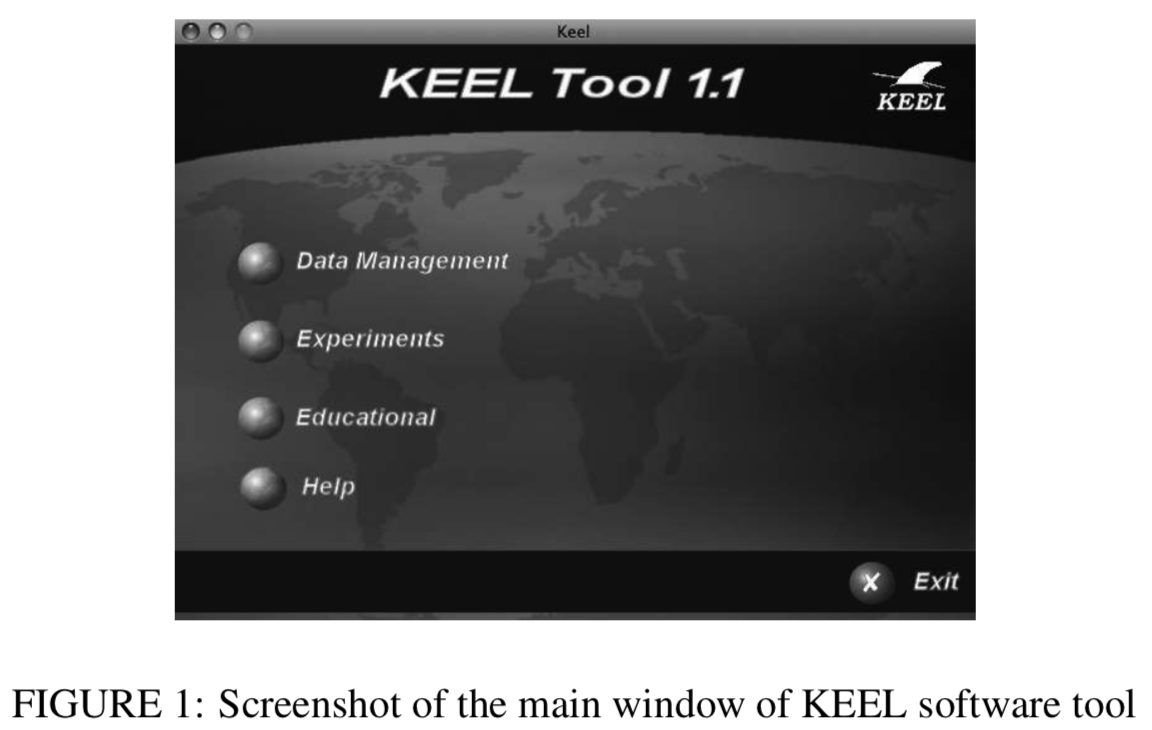
\includegraphics[width=1\linewidth]{./1.png}
\end{center}
\end{frame}

%------------------------------------------------
%------------------------------------------------

\begin{frame}
	\frametitle{\insertsection : \insertsubsection}
	\begin{block}{function blocks }
	\begin{itemize}
		\item Data Management
		\item Design of Experiments
		\item Educational Experiments
	\end{itemize}
	\end{block}
\end{frame}

%------------------------------------------------
%------------------------------------------------

\begin{frame}
	\frametitle{\insertsection : \insertsubsection}
	\begin{block}{main features of KEEL }
		\begin{itemize}
			\item  It presents \textbf{a large collection of EAs} for predicting models,\textbf{pre-processing  and post-processing}. 
			\\It also contains some state-of-the-art methods for\textbf{ different areas of DM} such as\textbf{ decision trees, fuzzy rule based systems or interval rule-based learning}.
			\item It has \textbf{a statistical library} to analyze results of algorthms.
			\item Some algorithms have been developed using \textbf{Java Class Library for Evolutionary Computation (JCLEC)} [43].
			\item The software is aimed at \textbf{creating experiments containing multiple data sets} and algorithms connected among themselves to \textbf{obtain an expected results}.
			\item KEEL also allows \textbf{the creation of experiments in on-line mode}, aiming to provide an educational support in order to \textbf{learn the operation of the algorithm} included.
		\end{itemize}
	\end{block}
\end{frame}

%------------------------------------------------
\section{KEEL-DATASET} 
%------------------------------------------------

\begin{frame}
	\frametitle{\insertsection : \insertsubsection}
	\begin{block}{In this section we present the KEEL-dataset repository. }
		\begin{itemize}
			\item A detailed categorization of the considered data sets and a description of their characteristics. \textbf{Tables for the data sets in each category have been also created.}
			\item A descriptions of the papers which have used the partitions of data sets available in the KEEL-dataset repository. These descriptions include \textbf{results tables, the algorithms used and additional material}.
		\end{itemize}
	\end{block}
\end{frame}

%------------------------------------------------
\subsection{Data sets webpages}
%------------------------------------------------

\begin{frame}
	\frametitle{\insertsection : \insertsubsection}
	The categories of the data sets have been derived from the topics addressed in the experimental studies.
\begin{center}
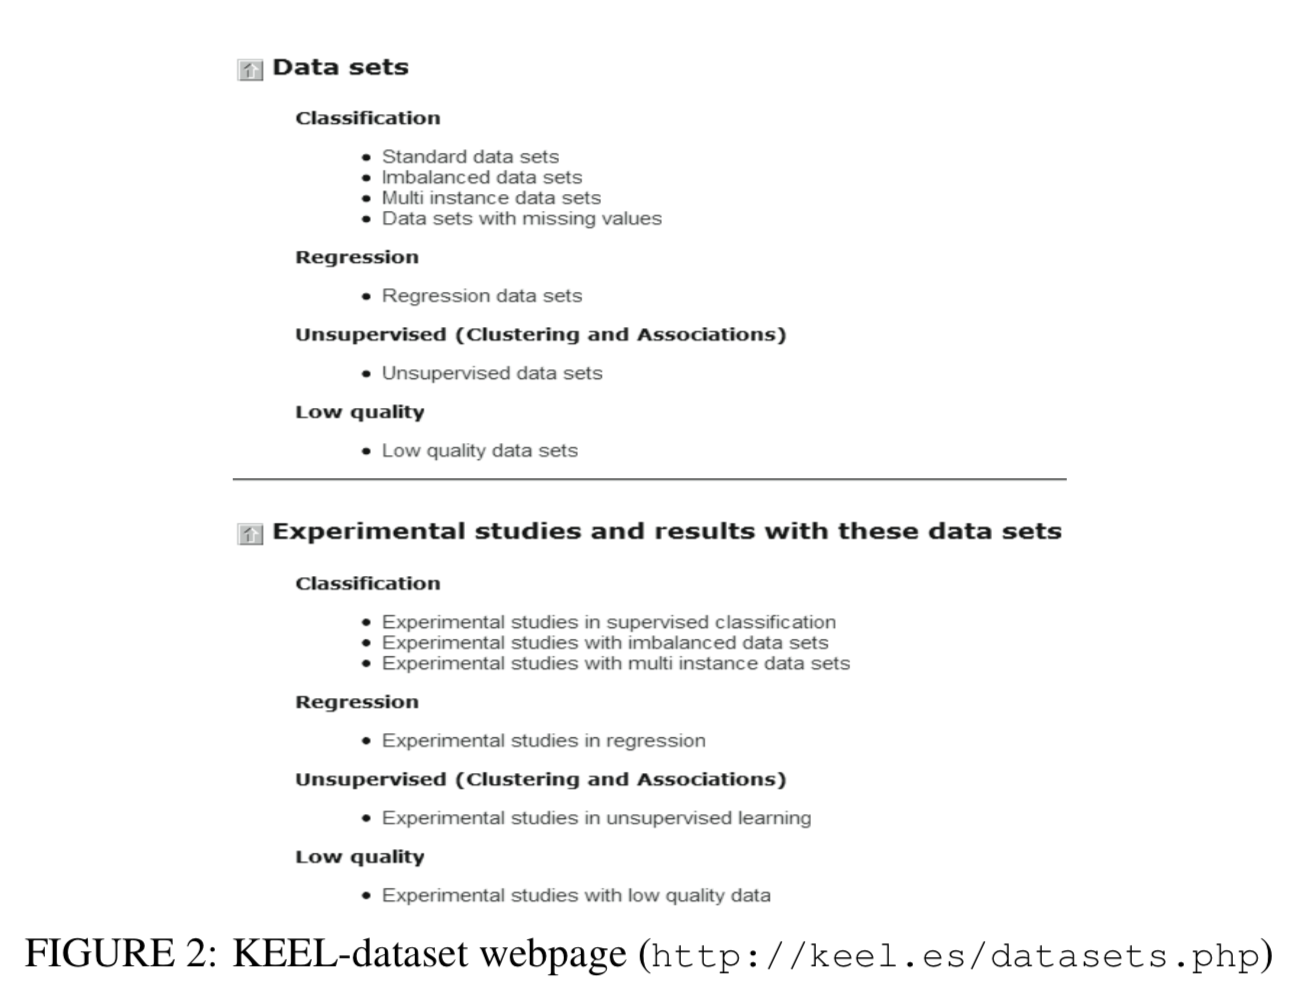
\includegraphics[ height=.75\textheight]{./2.png}
\end{center}
\end{frame}

%------------------------------------------------
%------------------------------------------------

\begin{frame}
	\frametitle{\insertsection : \insertsubsection}
	\begin{block}{The categories in which the data sets are divided are the following: }
		1.	Classification problems.
		\begin{itemize}
			\item Standard data sets.
			\item Imbalanced data sets [6, 28, 41].
			\item Multi instance data sets [12].
			\item Data sets with missing values.
		\end{itemize}
		2.	Regression problems.\\
		3.	Unsupervised (Clustering and Associations) problems.\\
		4.	Low quality data [37].
	\end{block}
\end{frame}

%------------------------------------------------
\subsection{Experimental study webpages}
%------------------------------------------------

\begin{frame}
	\frametitle{\insertsection : \insertsubsection}

	\begin{center}
		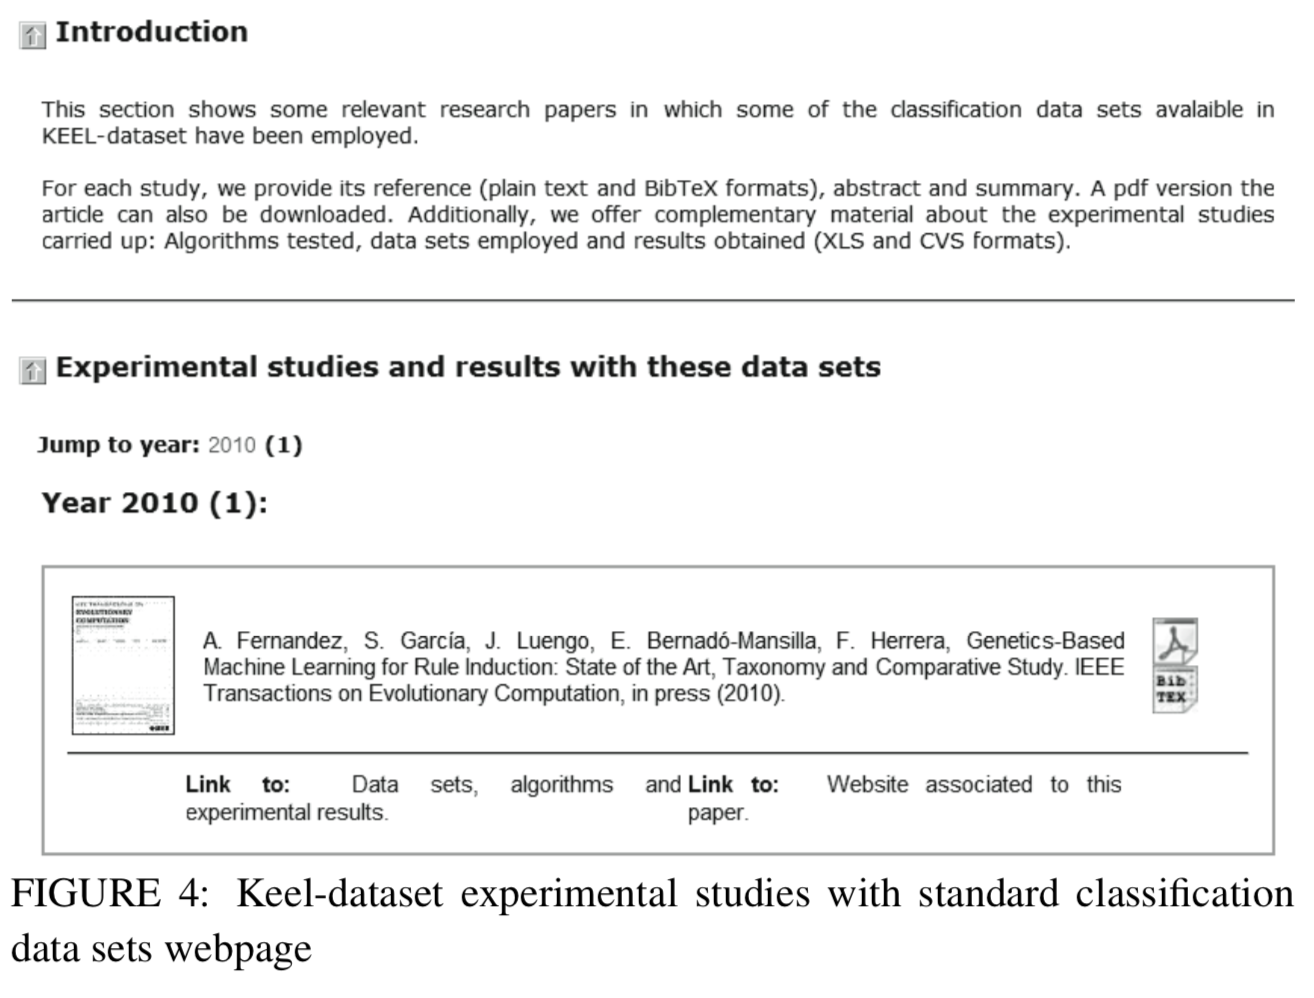
\includegraphics[ height=.85\textheight]{./3.png}
	\end{center}
\end{frame}

%------------------------------------------------
%------------------------------------------------

\begin{frame}
	\frametitle{\insertsection : \insertsubsection}
	
	\begin{block}{Each paper can contain up to four links: }
		These webpages contains \textbf{published journal publications} which use the correspondent kind of data sets in the repository.
		\begin{itemize}
			\item The first link is the PDF file of the paper.
			\item The second link is the Bibtex reference of the paper.
			\item At the bottom on the left link Data sets, algorithms and experimental results is always present. It references to the particular Keel-dataset webpage for such paper.
			\item At the bottom on the right link Website associated to this paper is only present for some papers which have a particular and external webpage related with them.
		\end{itemize}
	Moreover, the results are detailed and listed in CSV and XLS (Excel) formatted files.
	\end{block}
\end{frame}

%------------------------------------------------
\section{INTEGRATION OF NEW ALGORITHMS INTO THE KEEL TOOL} 
\subsection{Introduction to the KEEL codification features}

%------------------------------------------------

\begin{frame}
	\frametitle{\insertsection : \insertsubsection}
	

		\begin{itemize}
			\item The KEEL philosophy tries to include the fewest possible constraints for the developer, in order to ease the inclusion of new algorithms within this tool.
			\item We enumerate the list of details to take into account before codifying a method for the KEEL software, which is also detailed at the KEEL Reference Manual (http://www.keel.es/documents/KeelReferenceManualV1.0.pdf).
		\end{itemize}

\end{frame}

%------------------------------------------------

%------------------------------------------------

\begin{frame}
	\frametitle{\insertsection : \insertsubsection}
	
	
	\begin{itemize}
		\item The programming language used is Java.
		\item In KEEL,every method uses a configuration file to extract the values of the parameters which will be employed during its execution.
	\end{itemize}
		\begin{block}{Each configuration file has the following structure: }
			\begin{itemize}
				\item algorithm: Name of the method.
				\item inputData: A list with the input data files of the method.
				\item outputData: A list with the output data files of the method.
				\item parameters: A list of parameters of the method, containing the name of each parameter and its value (one line is employed for each one).
			\end{itemize}
		\end{block}
	
\end{frame}

%------------------------------------------------
%------------------------------------------------

\begin{frame}
	\frametitle{\insertsection : \insertsubsection}
	
\begin{center}
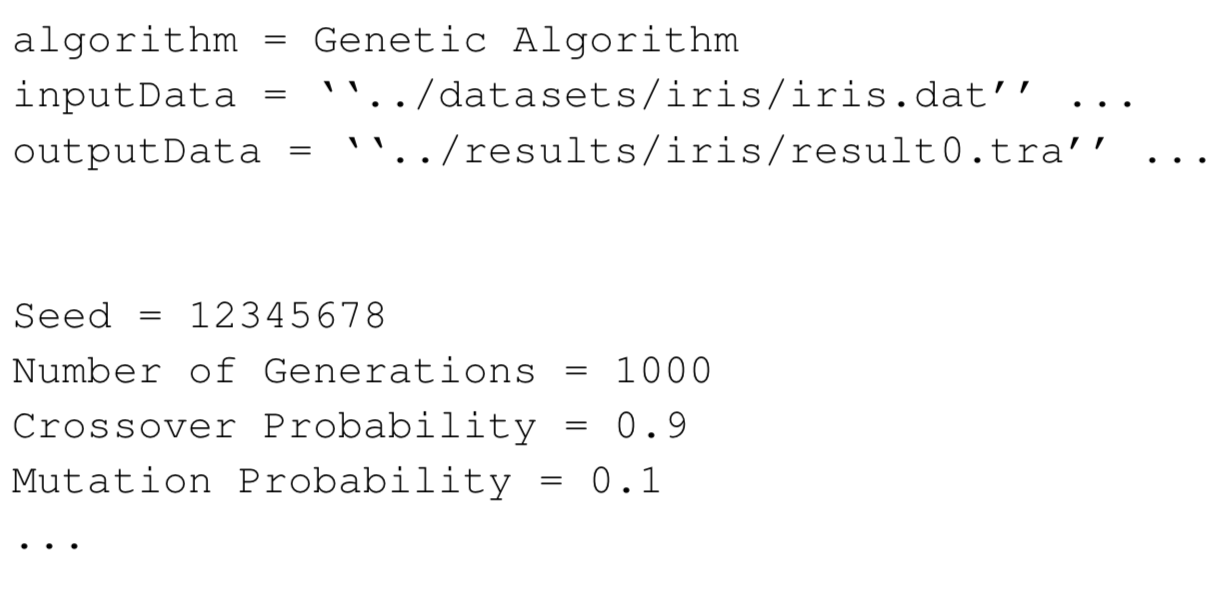
\includegraphics[width=1\linewidth]{./4.png}
\end{center}
\end{frame}

%------------------------------------------------
%------------------------------------------------

\begin{frame}
	\frametitle{\insertsection : \insertsubsection}
	
	
	\begin{itemize}
		\item The input data-sets follow a specific format that \textbf{extends the “arff” files} by completing \textbf{the header with more metadata information} about the attributes of the problem.
		\item The output format consists of a header,which\textbf{ follows the same scheme }as the input data, and two columns with the output values for each example separated by a whitespace.
	\end{itemize}

	
\end{frame}

%------------------------------------------------
%------------------------------------------------

\begin{frame}
	\frametitle{\insertsection : \insertsubsection}
	
	
	\begin{itemize}
		\item Although the list of constraints is short, the KEEL development team have created a simple template that \textbf{manages all these features}.
	\end{itemize}
	\begin{block}{Our KEEL template includes four classes}
		\begin{itemize}
{\small 		\item \textbf{Main}: This class contains the main instructions for launching the algorithm. 
			\item \textbf{ParseParameters}: This class manages all the parameters, from the input and output files, to every single parameter stored in the parameters file.
			\item \textbf{myDataset}: This class is an interface between the classes of the API data-set and the algorithm.
			\item \textbf{Algorithm}: This class is devoted to storing the main variables of the algorithm and to naming the different procedures for the learning stage.}
		\end{itemize}
	\end{block}
	
\end{frame}

%------------------------------------------------
%------------------------------------------------

\begin{frame}
	\frametitle{\insertsection : \insertsubsection}
	
	
	\begin{itemize}
		\item The template can be downloaded following the link \textbf{http://www.keel.es/software/KEEL\_template.zip}, which additionally supplies the user with the whole API data-set together with the classes for managing files and the random number generator.
	\end{itemize}
	
\end{frame}

%------------------------------------------------
\subsection{Encoding example using the “Steady-State Genetic Algorithm for Extracting Fuzzy Classification Rules From Data” method}

%------------------------------------------------

\begin{frame}
	\frametitle{\insertsection : \insertsubsection}
	
	
	\begin{itemize}
		\item We will show \textbf{how this template enables the programming within KEEL} to be straightforward, since the \textbf{user does not need to pay attention to the specific KEEL constraints} because they are completely covered by the functions\textbf{ implemented in the template.}
		\item To illustrate this, we have selected one classical and simple method, the SGERD procedure [33].
	\end{itemize}
	
\end{frame}

%------------------------------------------------
%------------------------------------------------

\begin{frame}
	\frametitle{\insertsection : \insertsubsection}
	
	
	\begin{itemize}
		\item Neither the \textbf{Main} nor the \textbf{ParseParameters }classes need to be modified, and we just need\textbf{ to focus }our attention on\textbf{ the Algorithm class }and the inclusion of \textbf{two new functions in myDataset}. 
		\item We enumerate below the steps for adapting this class to this specific algorithm:
	\end{itemize}
	
\end{frame}

%------------------------------------------------

\begin{frame}
	\frametitle{\insertsection : \insertsubsection}
	
		\begin{block}{1.}
	\begin{itemize}
		\item we must store all the parameters values with in the constructor of the algorithm. Each parameter is selected with the \textbf{getParameter} function using its corresponding position in the parameter file, whereas the optional output files are obtained using the function \textbf{getOutputFile}. 
		\item Furthermore, the constructor must check the capabilities of the algo- rithm, related to the data-set features, that is, whether it has missing values, real or nominal attributes, and so on.
	\end{itemize}
\end{block}
	
\end{frame}
%------------------------------------------------
%------------------------------------------------

\begin{frame}
	\frametitle{\insertsection : \insertsubsection}
	
	\begin{block}{2.}
		\begin{itemize}
			\item we execute the main process of the algorithm(procedure execute). 
			\item If everything is alright, we perform the algorithm’s operations.
			\item In the case of the SGERD method we must first build the Data Base (DB) and then generate an initial Rule Base (RB).
			\item Next, the GA is executed in order to find the best rules in the system.
		\end{itemize}
	\end{block}
	
\end{frame}
%------------------------------------------------
%------------------------------------------------

\begin{frame}
	\frametitle{\insertsection : \insertsubsection}
	
	\begin{block}{3.}
		\begin{itemize}
			\item We write in an output file the DB and the RB to save the generated fuzzy model, and then we continue with the classification step for both the validation and test files.
			\item The \textbf{doOutput} procedure simply iterates all examples and returns the predicted class as a string value (in regression problems it will return a double value). 
			\item This prediction is carried out in the \textbf{classificationOutput }function, which only runs the Fuzzy Reasoning Method of the generated RB (noted in boldface)
		\end{itemize}
	\end{block}
	
\end{frame}
%------------------------------------------------
%------------------------------------------------

\begin{frame}
	\frametitle{\insertsection : \insertsubsection}
	
	\begin{block}{4.}
		\begin{itemize}
			\item Finally, we show the new functions that are implemented in the \textbf{myDataset} class in order to obtain some necessary information from the training data during the rule learning stage. 
			\item We must point out that the remaining functions of this class remain unaltered.
		\end{itemize}
	\end{block}
	
\end{frame}
%------------------------------------------------
%------------------------------------------------

\begin{frame}
	\frametitle{\insertsection : \insertsubsection}
	

		\begin{itemize}
			\item Once the algorithm has been implemented, it can be executed directly on a terminal with the parameters file as an argument.
			\item Nevertheless, when included within the KEEL software, the user can create a complete experiment with automatically generated scripts for a batch-mode execution.
			\item Furthermore, we must clarify that the “validation file” is used when an instance- selection preprocessing step is performed, and contains the original training set data; hence, the training and validation files match up in the remaining cases.
		\end{itemize}

	
\end{frame}
%------------------------------------------------
%------------------------------------------------

\begin{frame}
	\frametitle{\insertsection : \insertsubsection}
	
	
	\begin{itemize}
		\item Finally, we should point out that the complete source code for the SGERD method (together with the needed classes for the fuzzy rule generation step)
can be downloaded at \textbf{http://www.keel.es/software/SGERD\_source. zip}.
	\end{itemize}
	
	
\end{frame}
%------------------------------------------------
\section{STATISTICAL TOOLS AND EXPERIMENTAL STUDY} 

%------------------------------------------------

\begin{frame}
	\frametitle{\insertsection : \insertsubsection}
	
	
	\begin{itemize}
		\item One of the important features of the KEEL software tool is the availability of a complete package of statistical procedures, developed with the aim of providing to\textbf{ the researcher a suitable tool to contrast the results obtained in any experimental study performed }inside the KEEL environment.
	\end{itemize}
	
	
\end{frame}
%------------------------------------------------
\subsection{KEEL Statistical Tests}
%------------------------------------------------

\begin{frame}
	\frametitle{\insertsection : \insertsubsection}
	
	
	\begin{itemize}
		\item Nowadays, the use of statistical tests \textbf{to improve the evaluation process of the performance of a new method }has become a widespread technique in the field of Data Mining [10, 19, 20]. 
		\item Usually, they are employed inside the framework of any experimental analysis \textbf{to decide} when an algorithm is better than other one.
		\item This task, which may not be trivial, has become necessary to confirm when a new proposed method \textbf{offers a significant improvement over the existing methods} for a given problem.
	\end{itemize}
	
	
\end{frame}
%------------------------------------------------
%------------------------------------------------

\begin{frame}
	\frametitle{\insertsection : \insertsubsection}
	
	
	\begin{itemize}
		\item There exist two kinds of test: \textbf{parametric} and \textbf{non-parametric}, depending of the concrete type of data employed. 
		\item As a general rule, a non-parametric test \textbf{is less restrictive than} a parametric one, although it is less robust than a parametric when data are well conditioned.
		\\
		\item Parametric tests have been commonly used in the analysis of experiments in DM.
		\item Nonparametric tests can be employed in the analysis of experiments, providing to the researcher a practical tool to use when the previous assumptions can not be satisfied.
	\end{itemize}
	
	
\end{frame}
%------------------------------------------------
%------------------------------------------------

\begin{frame}
	\frametitle{\insertsection : \insertsubsection}
	
	
	\begin{itemize}
		\item Table 1 shows the procedures existing in the KEEL statistical package. For each test, a reference and a brief description is given (an extended description can be found in the Statistical Inference in Computational Intelligence and Data Mining website and in the KEEL website  ).
	\end{itemize}
	
	
\end{frame}
%------------------------------------------------
%------------------------------------------------

\begin{frame}
	\frametitle{\insertsection : \insertsubsection}
	
	\begin{center}
		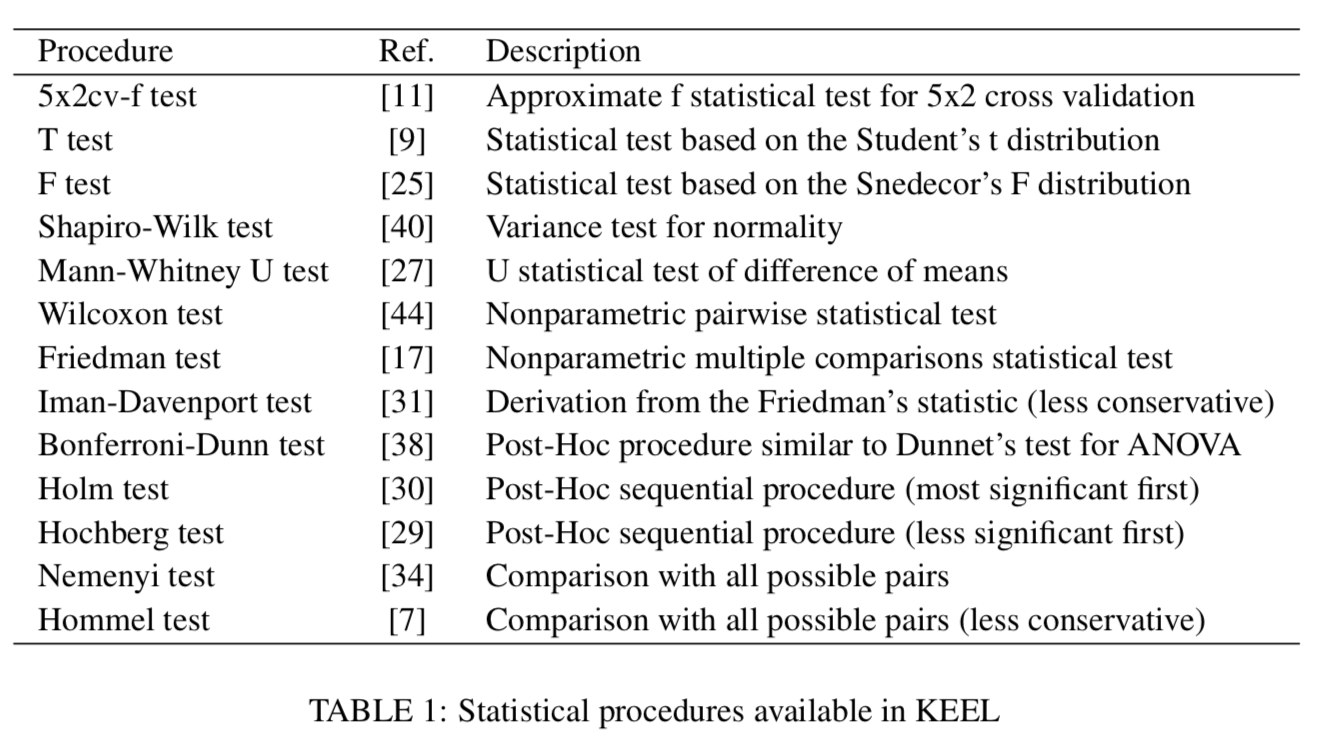
\includegraphics[width=1\linewidth]{./5.png}
	\end{center}
\end{frame}

%------------------------------------------------
\subsection{Case of study}
%------------------------------------------------

\begin{frame}
	\frametitle{\insertsection : \insertsubsection}
	
	
	\begin{itemize}
		\item In this section, we present a case study as an example of the functionality and process of creating an experiment with the KEEL software tool.
		\item This experimental study is focused on the comparison between the new algorithm imported (SGERD) and several evolutionary rule-based algorithms, and employs a set of supervised classification domains available in KEEL-dataset.
		\item Several statistical procedures available in the KEEL software tool will be employed to contrast the results obtained.
	\end{itemize}
	
	
\end{frame}
%------------------------------------------------
%------------------------------------------------

\begin{frame}
	\frametitle{\insertsection : \insertsubsection}
	\textbf{Algorithms and classification problems}
	
	\begin{itemize}
		\item \textbf{Five representative evolutionary rule learning methods} have been selected to carry out the experimental study: Ant-Miner, CO-Evolutionary Rule Extractor (CORE), HIerarchical DEcision Rules (HIDER), Steady-State Genetic Algorithm for Extracting Fuzzy Classification Rules From Data (SGERD) and \textbf{Tree Analysis }with Randomly Generated and Evolved Trees (TARGET) methodology.
	\end{itemize}
	
	
\end{frame}
%------------------------------------------------
%------------------------------------------------

\begin{frame}
	\frametitle{\insertsection : \insertsubsection}
	
	\begin{center}
		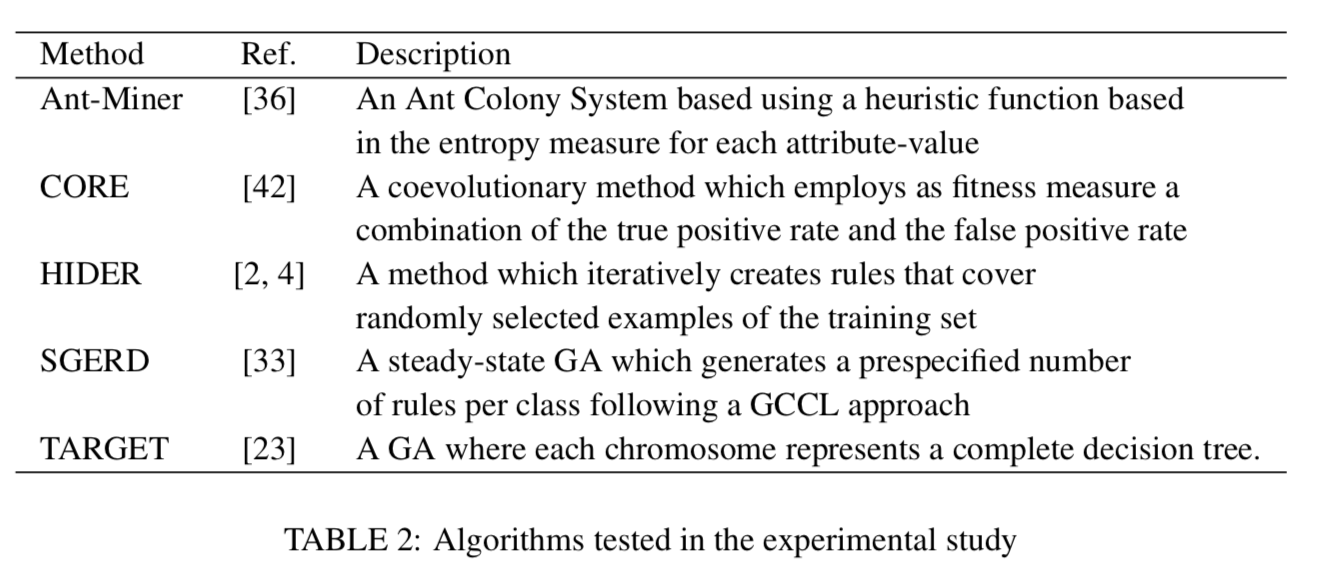
\includegraphics[width=1\linewidth]{./6.png}
	\end{center}
\end{frame}

%------------------------------------------------
%------------------------------------------------

\begin{frame}
	\frametitle{\insertsection : \insertsubsection}
	
	\begin{center}
		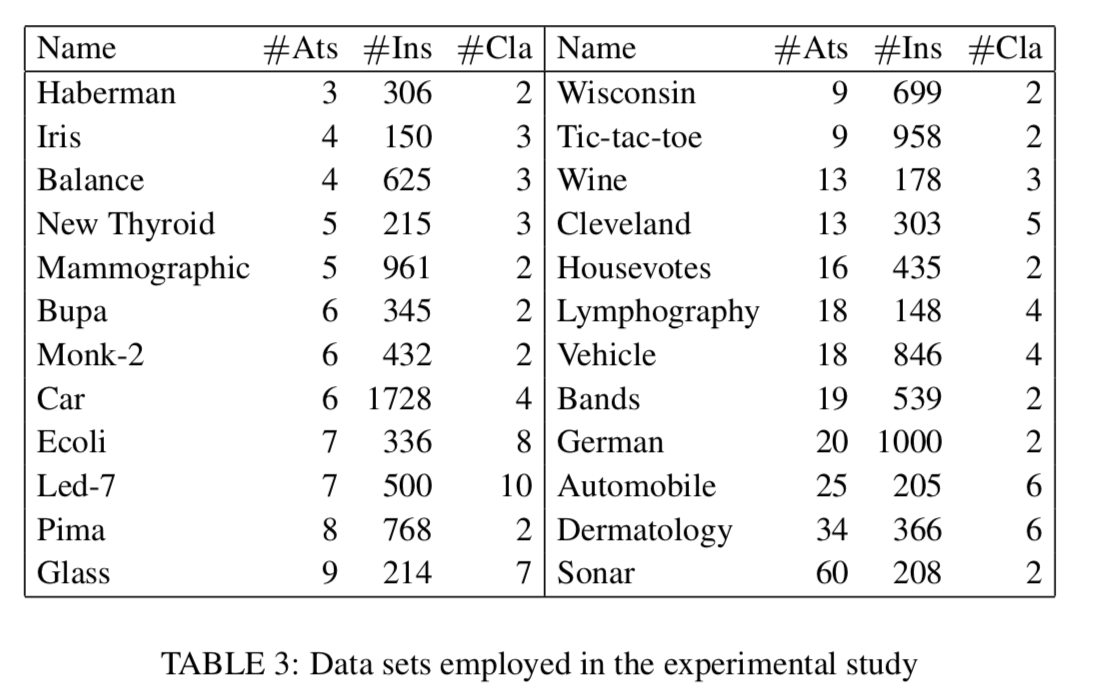
\includegraphics[width=.9\linewidth]{./7.png}
	\end{center}
\end{frame}

%------------------------------------------------
%------------------------------------------------

\begin{frame}
	\frametitle{\insertsection : \insertsubsection}
	\textbf{Setting up the Experiment under KEEL software}
	
	\begin{itemize}
		\item The graph in Figure 6 represents the flow of data and results from the algorithms and statistical techniques. 
		\item A node can represent an initial data flow (group of data sets), a pre-process/post-process algorithm, a learning method, test or a visualization of results module. 
		\item They can be distinguished easily by the color of the node. 
		\item All their parameters can be adjusted by clicking twice on the node. 
		\item Notice that KEEL incorporates the option of configuring the number of runs for each probabilistic algorithm, including this option in the configuration dialog of each node (3 in this case study).
	\end{itemize}
	
	
\end{frame}
%------------------------------------------------
%------------------------------------------------

\begin{frame}
	\frametitle{\insertsection : \insertsubsection}
	
	\begin{center}
		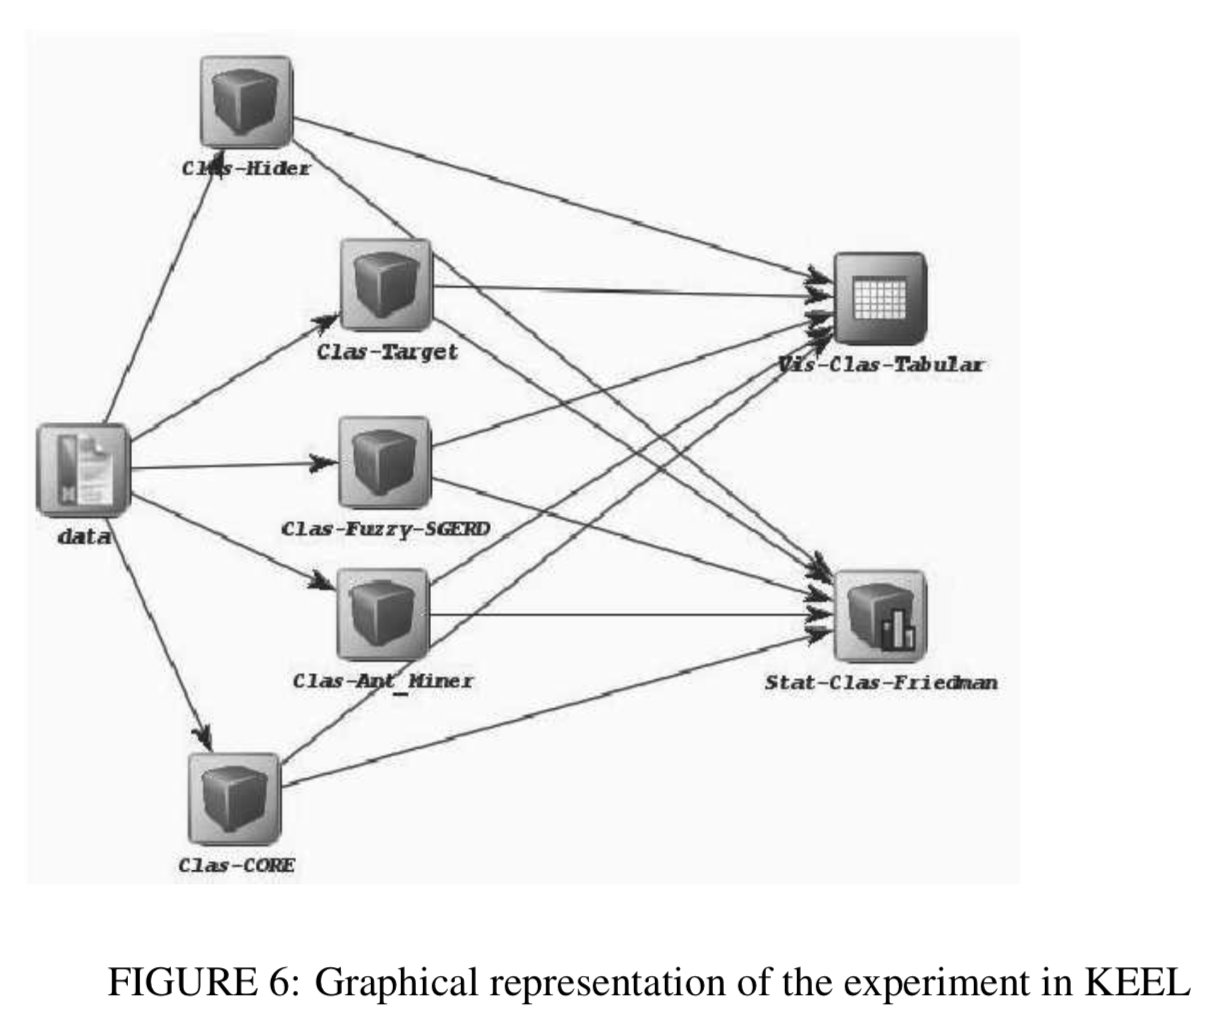
\includegraphics[width=.7\linewidth]{./8.png}
	\end{center}
\end{frame}

%------------------------------------------------
%------------------------------------------------

\begin{frame}
	\frametitle{\insertsection : \insertsubsection}
	
	\begin{itemize}
		\item Table 4 shows the parameter’s values selected for the algorithms employed in this experiment (they have been taken from their respective papers following the indications given by the authors).
	\end{itemize}
	
	
\end{frame}
%------------------------------------------------
%------------------------------------------------

\begin{frame}
	\frametitle{\insertsection : \insertsubsection}
	
	\begin{center}
		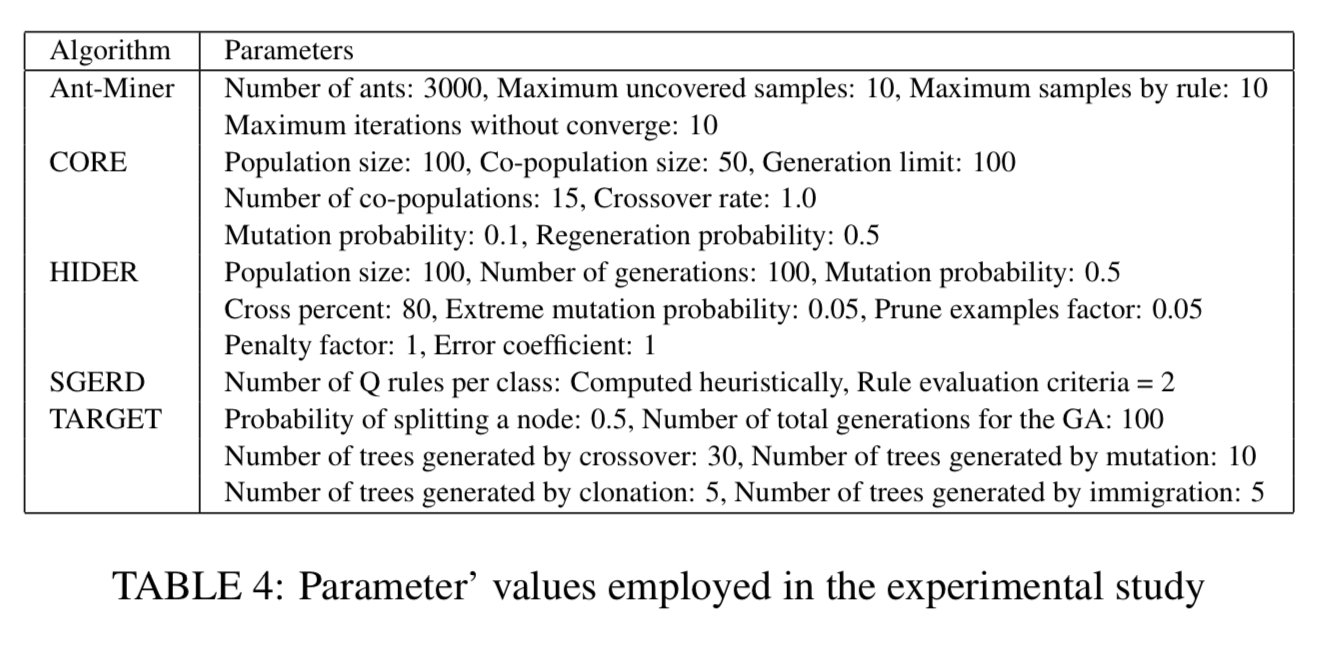
\includegraphics[width=1\linewidth]{./9.png}
	\end{center}
\end{frame}

%------------------------------------------------
%------------------------------------------------

\begin{frame}
	\frametitle{\insertsection : \insertsubsection}
	\textbf{Results and Analysis}
	
	\begin{itemize}
		\item This subsection describes and discusses the results obtained from the previous experiment configuration.
		\item Tables 5 and 6 show the results obtained in training and test stages, respectively. 
		\item For each data set, the average and standard deviations in accuracy obtained by the module Vis-Clas-Tabular are shown, with the best results stressed in \textbf{boldface}.
	\end{itemize}
	
	
\end{frame}
%------------------------------------------------
%------------------------------------------------

\begin{frame}
	\frametitle{\insertsection : \insertsubsection}
	
	\begin{center}
		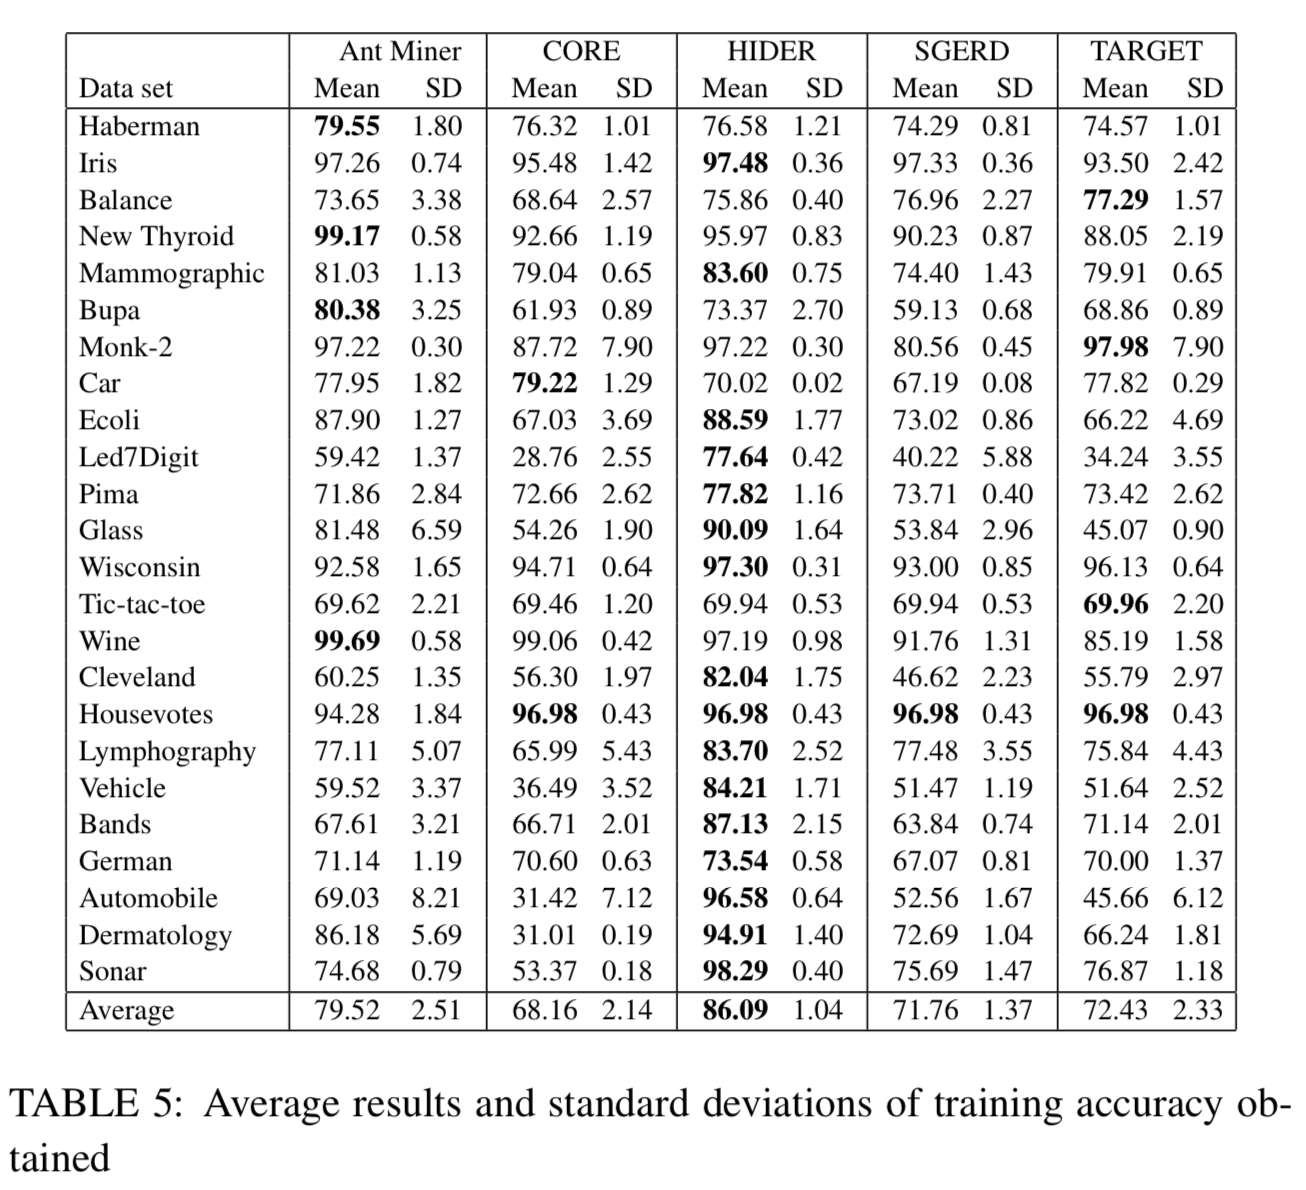
\includegraphics[width=.65\linewidth]{./10.png}
	\end{center}
\end{frame}

%------------------------------------------------
%------------------------------------------------

\begin{frame}
	\frametitle{\insertsection : \insertsubsection}
	
	\begin{center}
		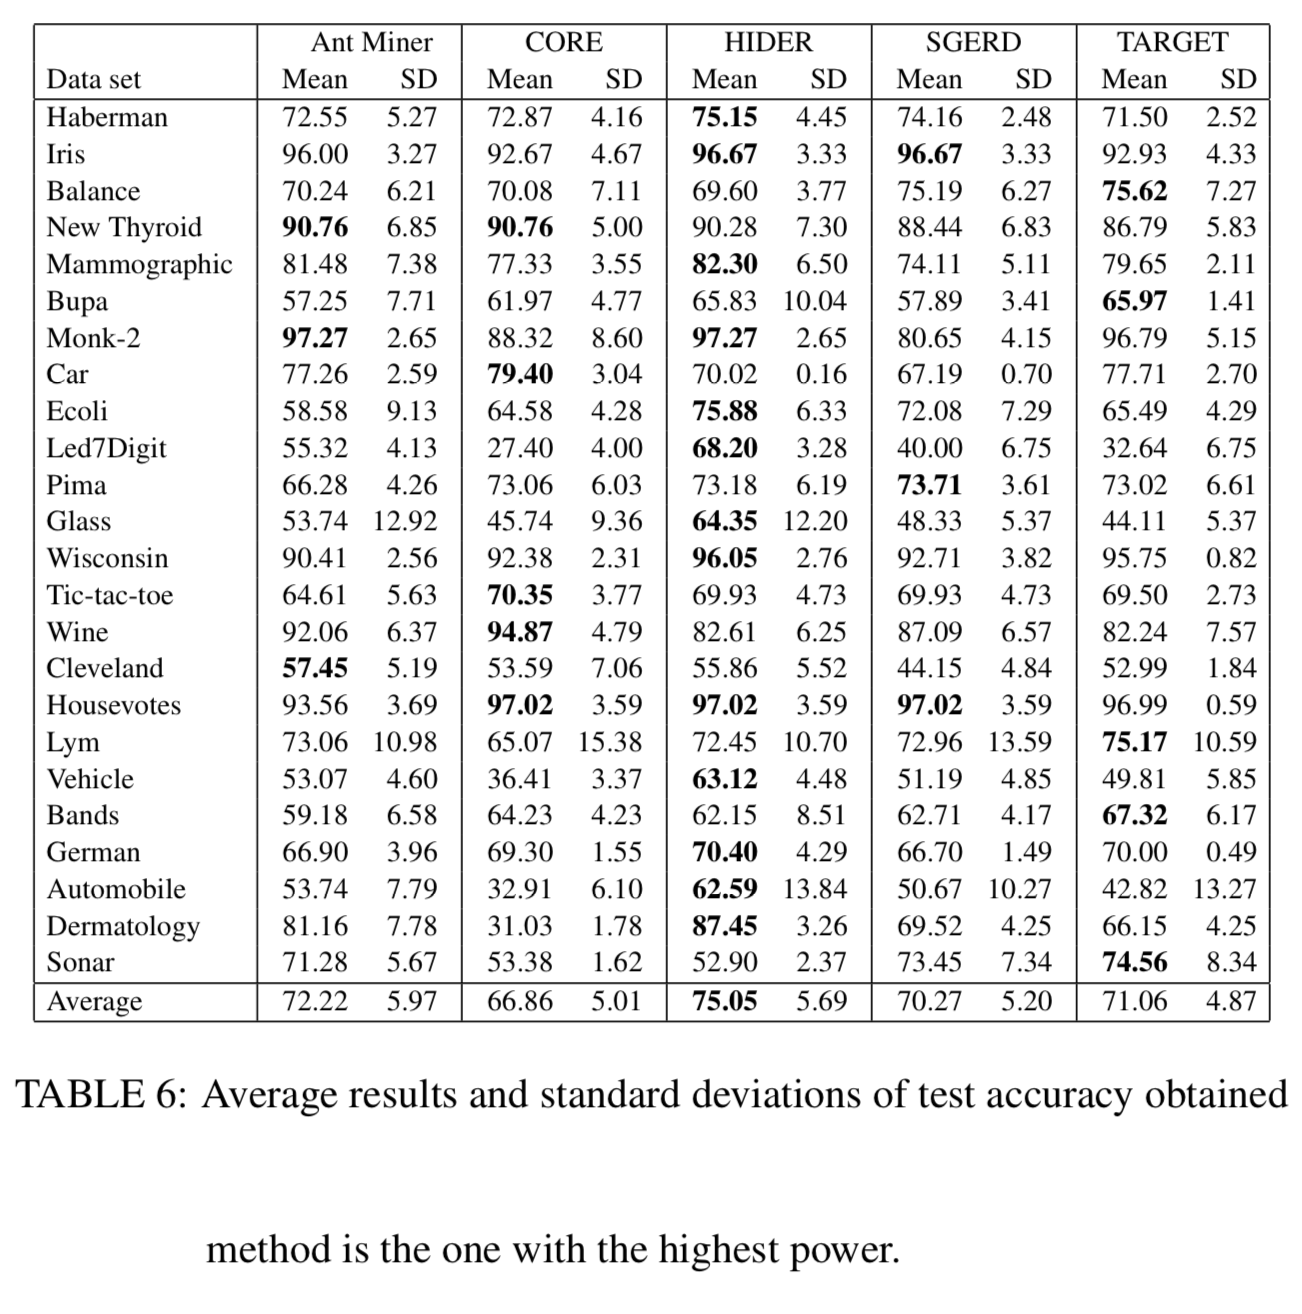
\includegraphics[width=.6\linewidth]{./11.png}
	\end{center}
\end{frame}

%------------------------------------------------
%------------------------------------------------

\begin{frame}
	\frametitle{\insertsection : \insertsubsection}

	
	\begin{itemize}
		\item Focusing on the test results, the average accuracy obtained by \textbf{Hider} is the highest one.
		\item However, this estimator does not reflect whether or not the differences among the methods are significant. 
		\item For this reason, we have carried out an statistical analysis based on multiple comparison procedures (see Appendix B for a full description), by including a node called Stat-Clas- Friedman in the KEEL experiment.
	\end{itemize}
	
	
\end{frame}
%------------------------------------------------
%------------------------------------------------

\begin{frame}
	\frametitle{\insertsection : \insertsubsection}
	
	\begin{center}
		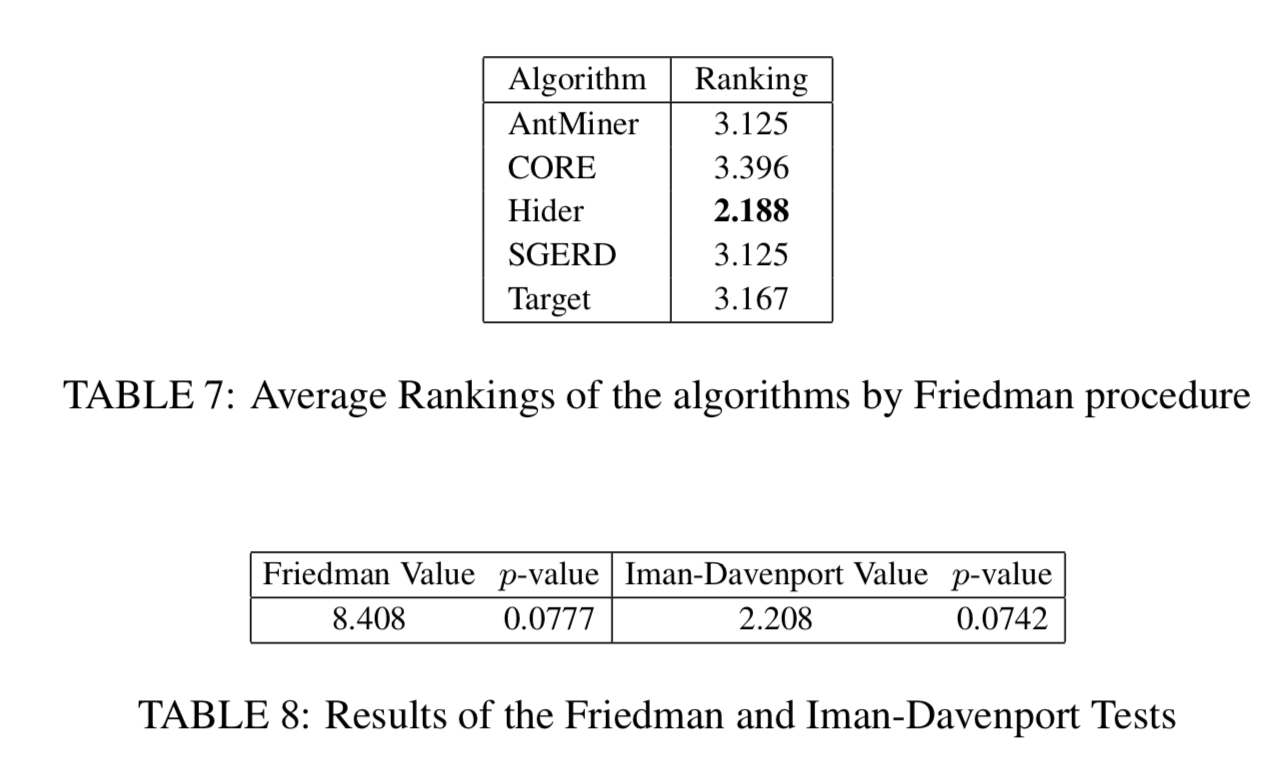
\includegraphics[width=1\linewidth]{./12.png}
	\end{center}
\end{frame}

%------------------------------------------------%------------------------------------------------

\begin{frame}
	\frametitle{\insertsection : \insertsubsection}
	
	\begin{center}
		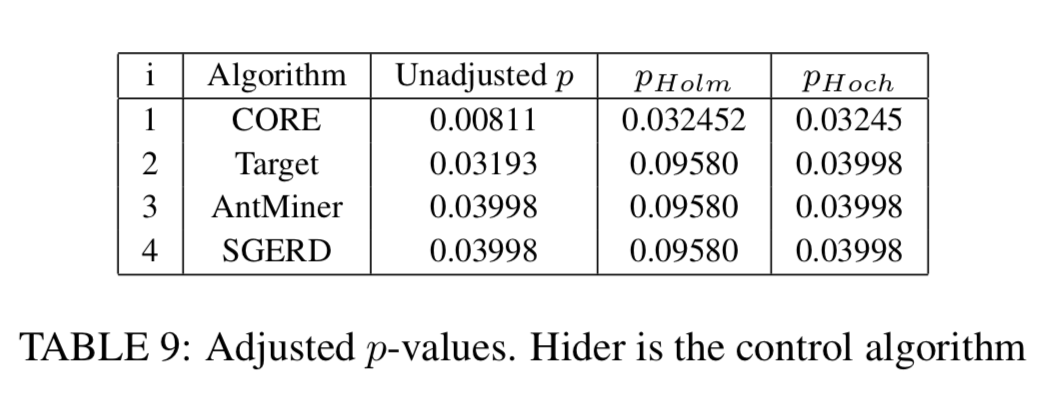
\includegraphics[width=1\linewidth]{./13.png}
	\end{center}
\end{frame}

%------------------------------------------------
\section{CONCLUDING REMARKS} 
%------------------------------------------------

\begin{frame}
	\frametitle{\insertsection : \insertsubsection}

	\begin{itemize}
		\item In this case, the results obtained have been contrasted through a statistical analysis following the indications given in [18], concluding that the Hider method is the best performing method when compared with the remaining methods analyzed in this study.
	\end{itemize}
	
	
\end{frame}
%------------------------------------------------
%------------------------------------------------

\begin{frame}
	\frametitle{\insertsection : \insertsubsection}
	The objective of this paper was to present three new aspects of KEEL:
	
	\begin{itemize}
		\item KEEL-dataset, a data set repository that includes the data set partitions in the KEEL format and shows some results obtained in these data sets.
		\item Some basic guidelines that the developer may take into account to facilitate the implementation and integration of new approaches within the KEEL software tool. 
		\item A module of statistical procedures which let researchers contrast the results obtained in any experimental study using statistical tests. This task, which may not be trivial, has become necessary to confirm when a new proposed method offers a significant i\textbf{mprovement over the existing methods} for a given problem.
	\end{itemize}
	
	
\end{frame}
%------------------------------------------------


\begin{frame}
\Huge{\centerline{Thank you for your attention}}
\end{frame}

%----------------------------------------------------------------------------------------

\clearpage\end{CJK*}
\end{document}